\section{Cadre mathématique.}

\subsection{Problème de Cauchy.}

Nous nous intéresserons au probème suivant, dit \emph{de Cauchy} :

\begin{equation}
  \label{eq:o1}
  y' = F(y,t),
\end{equation}
avec la condition initiale $y(t_{0})=y_{0}$,\\

%\clearslide{}
où:
\begin{itemize}
\item $y$ est l'inconnue ;
\item $y$ est une fonction dérivable définie sur un intervalle $I$ de $\R$ ;
\item $y$ et $F$ sont à valeurs dans $E = \R^{n}$ ou $E=\C^{n}$ ($n\in\N^{*}$) ;
\item $F$ est définie sur $E\times I$ ;
\item $t_{0}\in I$ et $y_{0}\in E$.
\end{itemize}

%\clearslide{}

\begin{rem}
En mathématiques et en physique, l'habitude est plutôt de considérer les équations 
différentielles sous la forme $y'=F(t,y)$ et non $y'=F(y,t)$.\\
Mais en Python, la fonction \texttt{odeint}, que nous verrons en fin de chapitre, 
utilise l'écriture $y'=F(y,t)$. Par souci de simplicité, nous nous conformerons à cette 
écriture dans ce cours.
\end{rem}


%\clearslide{}
\subsection{Notion de solution.}

On appelle \emph{solution} du problème précédent tout couple $(y,J)$ où :
\begin{itemize}
\item $J$ est un sous-intervalle de $I$ contenant $t_{0}$
\item $y : J\to E$ est une fonction dérivable vérifiant $y(t_{0})=y_{0}$ et
  \begin{equation*}
    \forall t \in J\quad y'(t)=F(y(t),t).
  \end{equation*}
\end{itemize}

On dit qu'une telle solution est \emph{maximale} s'il est
impossible de prolonger $y$ en une solution sur un intervalle strictement
plus grand que $J$.
%\clearslide{}

\subsection{Premier exemple : équation linéaire.}
Une solution de l'équation~(\ref{eq:o1}) avec la condition initiale $y(1)=2
\e$ où
\begin{equation*}
  F:\fct{\R\times \R}{\R}{(y,t)}{y}
\end{equation*}
est
\begin{equation*}
  \fct{[0,1]}{\R,}{t}{2 \e^{t},}
\end{equation*}
\emph{mais} cette solution n'est pas maximale car elle est prolongeable (par exemple) par
\begin{equation*}
  \fct{[0,17]}{\R,}{t}{2 \e^{t}.}
\end{equation*}
La seule solution maximale est dans ce cas:
\begin{equation*}
  \fct{\R}{\R,}{t}{2\e^{t}.}
\end{equation*}
%\clearslide{}

\subsection{Second exemple : équation non linéaire.}

On cherche à résoudre sur $\R$ l'équation
\begin{equation*}
  y' = \frac{3}{7}y^{3}
\end{equation*}
avec la condition initiale $y(0)=\frac{1}{36}$ :

\begin{itemize}
\item il n'y a pas de solution définie sur $\R$ tout entier (même en
  changeant la condition initiale, sauf pour une condition initiale $y(t_{0})=0$);
\item il y a une unique solution maximale: $t\mapsto\sqrt{\frac{7}{252 - 6t}}$;
\item cette solution maximale est définie sur $]-\infty, 42[$.
\end{itemize}
%\clearslide{}
\subsection{Théorème de Cauchy-Lipschitz.}

\emph{Sous des hypothèses raisonnables sur F :} pour chaque problème de Cauchy, il existe une unique solution
maximale.

\emph{Attention :} l'intervalle sur lequel une solution maximale est définie peut dépendre de
la condition initiale.

\subsection{En pratique}

Bien souvent, on considère en pratique le cas $I=[a,b]$ (où $a,b\in\R$ avec $a<b$) et les
solutions seront définies sur $I$ tout entier.

\emph{On se placera dans ce cadre pour la suite de ce cours.
On supposera que la condition initiale est donnée en $a$ et on notera
$y_{0}$ la valeur initiale de $y$ en $a$.
On note $y$ l'unique solution maximale du problème de Cauchy.}

\section{La méthode d'Euler.}

\subsection{Principe général.}

Nous avons vu en mathématiques que la résolution d'une équation différentielle linéaire du premier 
ordre se ramenait au calcul d'une primitive. Mais il existe des fonctions pour lesquelles nous ne 
savons pas calculer de primitive. Nous sommes donc incapables de résoudre ces équations de manière 
exacte. Quand il s'agit d'équations différentielles d'ordre supérieur ou non linéaires, la 
situation est encore moins favorable.

%\clearslide{}

Que faire s'il nous faut vraiment une solution à une telle équation différentielle ? Une 
possibilité est d'essayer d'obtenir une \emph{approximation numérique} d'une solution exacte. La 
méthode d'Euler est la méthode classique la plus simple pour faire cela. Le principe assez 
élémentaire de cette méthode est le suivant.

%\clearslide{}

On cherche à déterminer une approximation sur $[a,b]$ de la fonction $f : [a,b] \to \R$ vérifiant 
\begin{equation*}
  \forall t \in [a,b],~ f'(t) = F(f(t),t) \quad\textrm{et}\quad f(a) = y_0. 
\end{equation*}
On commence par choisir un \emph{pas} 
\begin{equation*}
  h=\frac{b-a}{n},
\end{equation*}
où $n\in\N^{*}$, et l'on subdivise l'intervalle $[a,b]$ en $n$ segments, en posant pour chaque $k\in \iif{0,n}$ :
\begin{equation*}
  t_{k} = a + k h = a + k \dfrac{b-a}{n}. 
\end{equation*}
Ainsi, $t_0 = a$ et $t_n = b$. On dit que $(t_0,\dots,t_n)$ est une subdivision régulière du segment $[a,b]$, avec $n+1$ points ou $n$ segments (ou morceaux). 

%\clearslide{}

On va ensuite construire $y_0,\dots,y_n$. L'approximation de la courbe de $f$ sera alors la ligne brisée reliant les points de coordonnées $(t_k,y_k)$. 

Le premier point $(t_0,y_0)$ est donné par la condition initiale. 

Pour chaque $k \in \ii{0,n}$, si les approximations $y_0,\dots,y_k$ aux temps $t_0,\dots,t_k$ sont construites, on approche la solution passant par le point de coordonnées $(t_k,y_k)$ par sa tangente. 
Comme la pente de cette tangente est $F(y_k,t_k)$, l'équation de cette tangente est alors 
\begin{equation*}
  y = y_k + F(y_k,t_k) (t-t_k). 
\end{equation*}
L'approximation de la solution au temps $t_{k+1}$ est alors (voir la figure~\ref{11:fig:principeEuler})
\begin{align*}
  y_{k+1} &= y_k + F(y_k,t_k) (t_{k+1}-t_k) \\
          &= y_k + hF(y_k,t_k).
\end{align*}

%\clearslide{}

% On espère alors que l'on aura $y_{k} \approx f(t_{k})$ pour tout $k \in \iif{1,n}$.

\begin{figure}[h!]
\begin{center}
\resizebox{0.8\textwidth}{!}{\input{images/euler-generique.pdf_t}}
\caption{Illustration du principe de la méthode d'Euler.}
\label{11:fig:principeEuler}
\end{center}
\end{figure}
%\clearslide{}

Par récurrence, on construit ainsi, de proche en proche, les réels $y_0$, $y_1$, $y_2$, $\cdots$, $y_n$ qui 
sont des approximations des $f(t_k)$. Chaque approximation $y_{k+1}$ est construite à partir de 
l'approximation précédente, $y_k$.

La ligne brisée joignant les points $(t_k,y_k)$ est le graphe d'une fonction, qui est elle-même une 
approximation de la solution exacte $f$.

\subsection{Premier exemple, une équation linéaire.}
On cherche à approcher la solution (maximale) sur $[0,3]$ de
\begin{equation*}
  y' = y
\end{equation*}
avec condition initiale $y(0)=1$.

\begin{rem}
  Vous savez bien entendu que c'est  $t\mapsto \e^{t}$.
\end{rem}

Numériquement, on regarde successivement les approximations obtenues par la méthode d'Euler avec les paramètres $n=3$, $n=30$ et $n=100$, soit des pas respectivement de $1$, $1/10$ et de $3/100$ (voir la figure~\ref{11:fig:exp3}).
\begin{figure}[h!]
\begin{center}
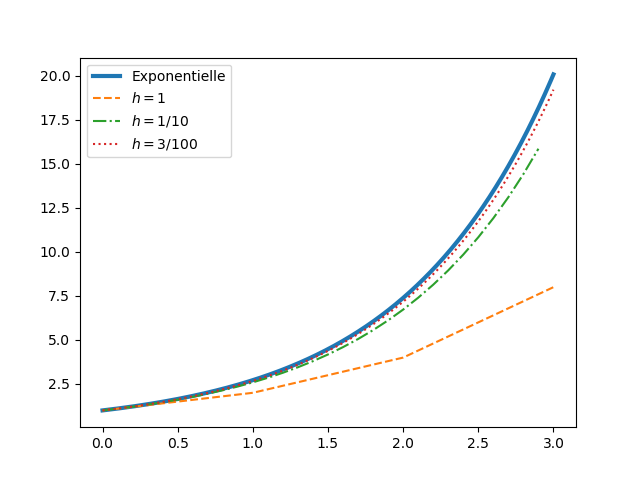
\includegraphics[width=\textwidth]{exp3.png}
\caption{Approximations de la solution du problème de Cauchy $y'=y$, $y(0)=1$ sur $[0,3]$.}
\label{11:fig:exp3}
\end{center}
\end{figure}

\subsection{Quelques remarques}
On peut conjecturer que
\begin{enumerate}
\item quand le pas diminue, l'approximation s'améliore;
\item la méthode d'Euler ne corrige pas les erreurs d'approximation
  mais au contraire les propage en les augmentant.
\end{enumerate}

En fait:
\begin{itemize}
\item Le premier point est vrai mathématiquement.
\item Le second dépend des équations considérées.
\end{itemize}

%\clearslide{}
Informatiquement:
\begin{itemize}
\item Si le pas est grand, l'approximation est mauvaise;
\item Si le pas est petit, elle est longue à calculer;
\item S'il est vraiment trop petit, les erreurs d'arrondis causent en
  plus d'autres problèmes.
\end{itemize}

%\clearslide{}
\section{Mise en œuvre.}

\subsection{Implantation de la méthode d'Euler.}

On traduit naïvement la méthode d'Euler. Cette fonction est extrêmement importante, vous devez savoir la reproduire.

\begin{pyverbatim}
def euler(F, a, b, y0, h):
    """Solution de y'=F(y,t) sur [a,b], y(a) = y0, pas h"""
    y = y0
    t = a
    y_list = [y0] # la liste des valeurs renvoyées
    t_list = [a] # la liste des temps
    while t+h <= b:
        # Variant : floor((b-t)/h)
        # Invariant : au tour k, y_list = [y_0,...,y_k], t_list = [t_0,...,t_k]
        y = y + h * F(y, t)
        y_list.append(y)
        t = t + h
        t_list.append(t)
    return t_list, y_list
\end{pyverbatim}
\begin{rem}
  Il est primordial d'utiliser ici l'écriture \pyv{y = y + h * F(y, t)} au lieu de  \pyv{y += h * F(y, t)}, qui ne donne pas le résultat escompté dans le cas vectoriel. 
\end{rem}

\begin{rem}
  La variante écrite au dessus correspond au cas où le pas $h$ nous est donné. 
  Si le nombre de subdivisions $n$ nous est donné à la place, on pourra préférer écrire la fonction avec une boucle \pyv{for}, en utilisant la fonction \pyv{linspace} du module \pyv{numpy}.
\end{rem}

\subsection{Exemple et représentation graphique.}

Problème de cinétique chimique : on s'intéresse à une réaction chimique
faisant disparaître un réactif $A$ d'une solution.

On suppose que la vitesse de disparition de $A$ est proportionnelle
à sa concentration (réaction d'ordre $1$). La concentration de $A$ suit donc l'équation
\begin{equation*}
  \dfrac{\textrm{d}[A]}{\textrm{dt}} = -\alpha [A],
\end{equation*}
où $\alpha$ est une constante s'exprimant en $s^{-1}$.% (la valeur $\frac{\ln 2}{\alpha}$ est un temps appelé temps de demi-réaction).

L'équation est bien de la forme
\begin{equation*}
  [A]' = F([A],t) \qquad \text{où }F : (y,t)\mapsto -\alpha y.
\end{equation*}

On suppose $\alpha=1$ (unité : $s^{-1}$) et, au temps $t=0$, $[A] =
1$ (unité : $mol.l^{-1}$). 
On étudie l'évolution sur l'intervalle de temps $[0,6]$ (unité : $s$).


Le code suivant permet de tracer (voir figure~\ref{11:fig:reaction_ordre1}) simplement la solution approchée par la méthode d'Euler pour le pas de $h=\dfrac{1}{10}$ (on considère que la fonction \pyv{euler} a déjà été écrite). 

\begin{pyverbatim}
import matplotlib.pyplot as plt

A0 = 1 # mol
alpha = 1 # s**-1
t0,t1,h = 0,6,.1

def F(y,t) :
    return -alpha*y

t_list,A_list = euler(F,t0,t1,A0,h)
plt.plot(t_list,A_list)
plt.xlabel('Temps ($s$)')
plt.ylabel('Concentration ($mol$)')
plt.grid()
plt.savefig('reaction_ordre1.png')
\end{pyverbatim}
\begin{figure}[!h]
    \begin{center}
        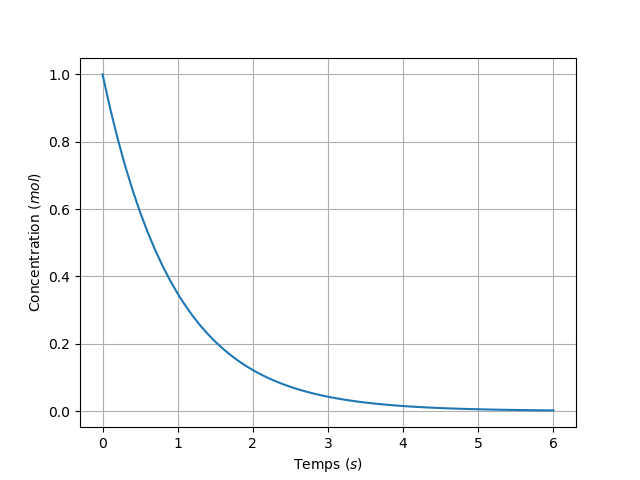
\includegraphics[width=\textwidth]{reaction_ordre1.png}
        \caption{Tracé de la trajectoire.}
        \label{11:fig:reaction_ordre1}
    \end{center}
\end{figure}

\section{Équations d'ordres supérieurs.}

\subsection{Dérivation de fonctions à valeurs vectorielles.}

En mathématiques et en physique, vous avez pris l'habitude de dériver des fonctions à valeurs complexes (et à variables réelles). 
Par exemple, si $z : \R\to\C$ a pour partie réelle $x$ et pour partie imaginaire $y$, alors si $z$ est dérivable on a 
\begin{equation*}
    z' = x' + iy'.
\end{equation*}
On procède de même pour dériver des fonctions à valeurs vectorielles (du moins, dans un espace de dimension finie !) : on dérive composante par composante. 
Ainsi, si une fonction $X : \R\to\R^2$ a pour composantes $x$ et $y$, \emph{i.e.} 
\begin{equation*}
    X : t \mapsto \bpm x(t) \\ y(t) \epm,
\end{equation*}
alors si $X$ est dérivable, on a 
\begin{equation*}
    X' : t \mapsto \bpm x'(t) \\ y'(t) \epm.
\end{equation*}

\subsection{Vecteurs numpy}

La bibliothèque numpy fournit le type \pyv{array} (vecteur, en anglais), qui permet d'effectuer directement du calcul vectoriel. 
Les vecteurs sont à distinguer des listes (même si ces deux types partagent certaines propriétés, comme le tranchage). Notamment, les vecteurs sont des données homogènes de taille fixée. 

\begin{pyconsole}
from numpy import array
v = array([1.,2.])
v
w = array([-5,2.5])
v + 3*w
\end{pyconsole}
On peut accéder aux coordonnées d'un vecteur avec les notations habituelles. 
\begin{pyconsole}
v[0],v[1]
\end{pyconsole}

\subsection{Vectorialisation d'équation différentielle.}

On donne ici l'exemple d'une équation différentielle d'ordre $2$ (le cas le plus courant que vous rencontrerez), cela se généralise sans peine aux ordres supérieurs. 

On considère un problème de Cauchy d'ordre $2$ : 
\begin{equation*}
    y''(t) = f(y(t),y'(t),t), \quad y(t_0) = y_0, y'(t_0) = z_0, 
\end{equation*}
défini sur un intervalle de temps $I$ et où $t_0\in I$. 

L'idée est alors de \emph{vectorialiser} cette équation, pour obtenir une équation \emph{d'ordre 1} sur une variable vectorielle de \emph{dimension 2}. 
Pour cela, on considère la variable 
\begin{equation*}
    X(t) = \bpm y(t) \\ y'(t) \epm.
\end{equation*}
On a alors 
\begin{equation*}
    X'(t) = \bpm y'(t) \\ y''(t) \epm = \bpm y'(t) \\ f(y(t),y'(t),t) \epm. 
\end{equation*}
Avec 
\begin{equation*}
    \fonction{F}{\R^2\times I}{\R^2}{\p{\bpm a\\b \epm , t }}{ \bpm b \\ f(a,b,t) \epm},
\end{equation*}
on obtient donc bien le problème de Cauchy équivalent : 
\begin{equation*}
    X'(t) = F(X(t),t) \quad\textrm{et}\quad X(t_0) = \bpm y_0 \\z_0 \epm. 
\end{equation*}

\begin{rem}
    On notera bien que la condition initiale de ce problème de Cauchy est vectorielle. 
\end{rem}

\subsection{Exemple : système ressort-amortisseur, tracé de la trajectoire et du portrait de phase.}

Considérons l'équation d'un système ressort-amortisseur : 
\begin{equation*}
  m y'' = - c y' - ky,
\end{equation*}
sur l'intervalle de temps $[0,20]$ (unité : $s$), avec les conditions initiales $y(0) = 1$ (unité : $m$) et $y'(0) = 0$ (unité : $m.s^{-1}$).

On vectorialise l'équation en considérant la variable 
\begin{equation*}
    X(t) = \bpm y(t) \\ y'(t) \epm,
\end{equation*}
l'équation s'écrit alors 
\begin{equation*}
    X'(t) = F(X(t),t)
\end{equation*}
avec 
\begin{equation*}
    \fonction{F}{\R^2\times [0,20] }{\R^2}{\p{\bpm a\\b \epm , t }}{ \bpm b \\ -\dfrac{ka+cb}{m} \epm}
\end{equation*}
et la condition initiale
\begin{equation*}
    X(0) = \bpm 1\\0 \epm. 
\end{equation*}


On considère les constantes suivantes : $m = 250$ (unité : $kg$), $k = 1000$ (unité : $kg.s^{-2}$) et $c = 100$ (unité : $kg.s^{-1}$).

Le script suivant permet d'appliquer la méthode d'Euler à l'équation vectorialisée (on suppose la fonction \pyv{euler} déjà écrite). 
\begin{pyverbatim}
y0 = 1 # m
yp0 = 0 # m * s**-1
t0, t1, h = 0, 20, .01 # s
m = 250 # kg
c = 100 # kg * s**-1
k = 1000 # kg * s**-2

def F(X,t) :
    y,yp = X
    ypp = -(k*y + c*yp)/m
    return array([yp,ypp])

X0 = array([y0,yp0])

t_list, X_list = euler(F,t0,t1,X0,h)
\end{pyverbatim}

\textsc{Attention !} La variable \pyv{X_list} est une liste de vecteurs ! On peut récupérer les positions et les vitesses comme suit. 

\begin{pyverbatim}
y_list = [X[0] for X in X_list]
yp_list = [X[1] for X in X_list]
\end{pyverbatim}

On trace ensuite simplement la trajectoire (position en fonction du temps, voir figure~\ref{11:fig:oscillateur_amorti_trajectoire}) et le portrait de phase (courbe (position,vitesse), voir figure~\ref{11:fig:oscillateur_amorti_phase}) comme suit. 
\begin{pyverbatim}
plt.clf()
plt.plot(t_list,y_list)
plt.xlabel('Temps ($s$)')
plt.ylabel('Position ($m$)')
plt.grid()
plt.savefig('oscillateur_amorti_trajectoire.png')

plt.clf()
plt.plot(y_list,yp_list)
plt.xlabel('Position ($m$)')
plt.ylabel('Vitesse ($m.s^{-1}$)')
plt.grid()
plt.savefig('oscillateur_amorti_phase.png')
\end{pyverbatim}
\begin{figure}[!h]
    \begin{center}
        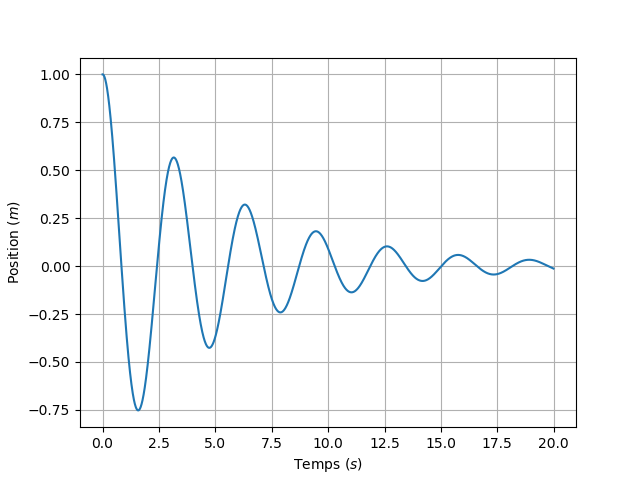
\includegraphics[width=\textwidth]{oscillateur_amorti_trajectoire.png}
        \caption{Oscillateur amorti, trajectoire par la méthode d'Euler.}
        \label{11:fig:oscillateur_amorti_trajectoire}
    \end{center}
\end{figure}
\begin{figure}[!h]
    \begin{center}
        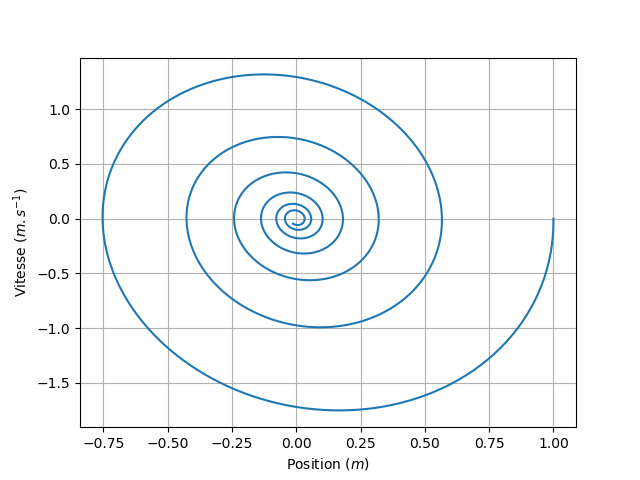
\includegraphics[width=\textwidth]{oscillateur_amorti_phase.png}
        \caption{Oscillateur amorti, portrait de phase par la méthode d'Euler.}
        \label{11:fig:oscillateur_amorti_phase}
    \end{center}
\end{figure}

%\clearslide{}
\section{Utilisation de scipy}

Nous ne sommes pas les seuls à vouloir résoudre numériquement des
équations différentielles, donc il doit déjà exister des implantations
pour ça.

Il existe de nombreux intérêt à réutiliser une implantation existante :
\begin{itemize}
\item gain de temps (pas besoin de la reprogrammer) ;
\item bugs connus (trouvés par d'autres) ;
\item problèmes de performance connus (remarqués par d'autres).
\end{itemize}

%\clearslide{}

De plus on peut espérer :
\begin{itemize}
\item que les bugs ont été corrigés ;
\item que les performances ont été optimisées.
\end{itemize}

Dans le cas du logiciel libre :
\begin{itemize}
\item c'est souvent le cas ; 
\item sinon, on peut réparer le logiciel soi-même (ou le faire réparer).
\end{itemize}

%\clearslide{}
La bibliothèque \pyv{scipy} propose un grand nombre de méthodes de calcul numérique. En particulier, \pyv{odeint} :
\begin{itemize}
\item est une fonction de la bibliothèque \pyv{scipy.integrate} ;
\item résout numériquement des EDO ;
\item utilise une méthode plus raffinée que celle d'Euler ;
\item fonctionne sur une équation vectorielle avec le type \pyv{array} ;
\item choisit elle-même le pas à utiliser.
\end{itemize}

%\clearslide{}
On l'utilise comme suit.
\begin{pyverbatim}
from scipy.integrate import odeint
y_list = odeint(F, y0, t_list)
\end{pyverbatim}

%\clearslide{}
Reprenons l'exemple de l'oscillateur amorti (voir le résultat figure~\ref{11:fig:oscillateur_amorti_odeint}).
\begin{pyverbatim}
from scipy.integrate import odeint
from numpy import linspace

y0 = 1 # m
yp0 = 0 # m * s**-1
t0, t1 = 0, 20 # s
n = 1000
m = 250 # kg
c = 100 # kg * s**-1
k = 1000 # kg * s**-2

X0 = array([y0,yp0])

def F(X,t) :
    y,yp = X
    ypp = -(k*y + c*yp)/m
    return array([yp,ypp])

t_list = linspace(t0,t1,n)
X_list = odeint(F,X0,t_list)
y_list = [X[0] for X in X_list]

plt.clf()
plt.plot(t_list,y_list)
plt.xlabel('Temps ($s$)')
plt.ylabel('Position ($m$)')
plt.grid()
plt.savefig('oscillateur_amorti_odeint.png')
\end{pyverbatim}


%\clearslide{}

\begin{figure}[!h]
    \begin{center}
        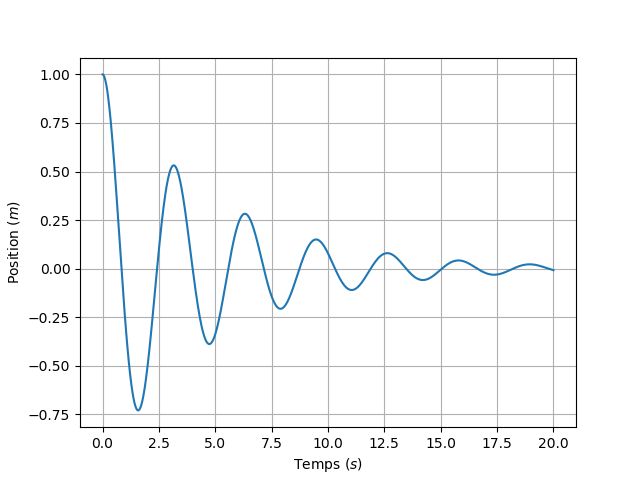
\includegraphics[width=\textwidth]{oscillateur_amorti_odeint.png}
        \caption{Oscillateur amorti, trajectoire par \texttt{odeint}.}
        \label{11:fig:oscillateur_amorti_odeint}
    \end{center}
\end{figure}
\textsc{Attention !} On ne donne pas les extrémités de l'intervalle mais les points  où l'on veut des valeurs, \pyv{y0} (condition initiale) est la valeur en
  \pyv{t_list[0]}.

%\clearslide{}


\section{Influence du pas de discrétisation}
On reprend l'exemple de l'amortisseur, avec $c=100$ et avec
différentes valeurs du pas de discrétisation $h$ (voir figure~\ref{11:fig:oscillateur_amorti_pas}).

\begin{figure}[!h]
    \begin{center}
        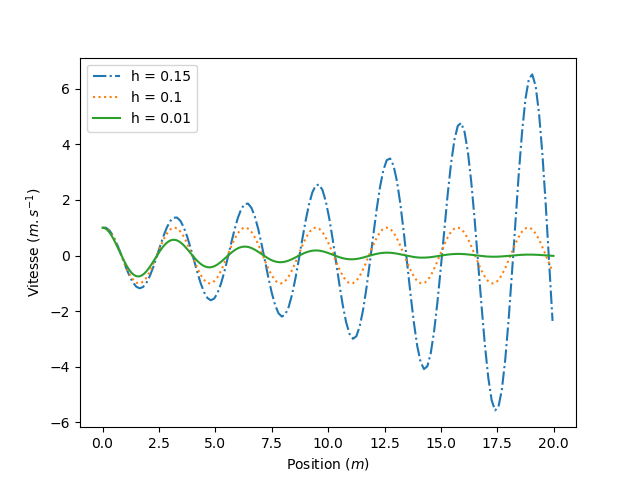
\includegraphics[width=\textwidth]{oscillateur_amorti_pas.png}
        \caption{Oscillateur amorti, trajectoires par la méthode d'Euler avec différents pas.}
        \label{11:fig:oscillateur_amorti_pas}
    \end{center}
\end{figure}

La première courbe est clairement délirante sur le plan physique...
Plusieurs facteurs contribuent à l'erreur~:

\begin{itemize}
\item des \emph{erreurs de méthode} (la méthode d'Euler n'est pas parfaite)
\item des \emph{erreurs de calcul} (les flottants ne sont pas les réels)
\end{itemize}

%\clearslide{}
Rappelons que pour un pas $h$ on note $n$ le nombre de morceaux utilisés. Pour les erreurs de méthode, on dit qu'il y a \emph{convergence} si :
\begin{enumerate}
\item la somme $e(h)=\displaystyle\sum_{k=0}^n |y(t_k)-y_k|$ des petites erreurs 
commises à 
chaque étape tend vers $0$ quand $h$ tend vers $0$ ($e(h)$ est appelée 
  \emph{erreur de consistance relative à la solution $y$}).
\item et certaines conditions de \emph{stabilité} de la méthode employée sont
  respectées (essentiellement, si l'on commet une petite erreur à chaque étape du calcul des $y_k$, 
  menant à de nouvelles approximations $\tilde{y}_k$, alors si l'erreur de consistance relative aux $y_k$
  est petite, l'erreur entre les $y_k$ et les $\tilde{y}_k$ doit être petite aussi).
\end{enumerate}

On dit qu'une méthode est d'\emph{ordre $p$} s'il existe une constante $K>0$ telle que
$e(h)\leq Kh^p$, autrement dit l'erreur de consistance est un $O(h^{p})$.

La méthode d'Euler est une méthode d'ordre $1$.


%\clearslide{}
\section{Annexe : autres méthodes.}
\subsection{Méthode d'Euler implicite}
La méthode d'Euler présentée jusqu'ici est dite \emph{explicite}~:
$y_{k+1}$ ne dépend que $y_k$ et $t_k$.

\begin{equation*}
 y_{k+1} = y_{k} + h F(y_{k},t_{k})
\end{equation*}

%\clearslide{}
Mais en reprenant les approximations qui ont conduit à ce schéma, 
nous pouvons aussi bien écrire~:
\begin{equation*}
 y_{k+1} = y_{k} + h F(y_{k+1},t_{k})
\end{equation*}


ce qui mène à la méthode d'Euler \emph{implicite}.

Elle a un gros inconvénient~: pour trouver $y_{k+1}$, il faut résoudre une équation
(numériquement).

Mais elle a un avantage~: elle est souvent plus stable.

\subsection{Méthode de Heun}

Si $y_{n} = y(t_{n})$, il existe $c\in]t_{n},t_{n+1}[$ tel que
\begin{equation*}
 y(t_{n+1}) = y_{n} + hy'(c) 
\end{equation*}

Tout le problème est d'estimer $y'(c)$.

%\clearslide{}

On connaît l'idée de la méthode d'Euler explicite~:
\begin{equation*}
  y'(c)\approx y'(t_{n})
\end{equation*}
Donc on pose $\boxed{k_{1}=F(y_{n},t_{n})}$.

Puis
\begin{equation*}
  \boxed{y_{n+1} = y_{n} + hk_{1}}
\end{equation*}
(erreur locale en $O(h^{2})$)

%\clearslide{}
L'idée de la méthode de Heun est la suivante~:
\begin{equation*}
  y'(c)\approx \frac{y'(t_{n})+y'(t_{n+1})}{2}
\end{equation*}
On pose $\boxed{k_{1} = F(y_{n},t_{n})}$.
Alors $k_{1} = y'(t_{n})$.

On estime $y'(t_{n+1})$ en utilisant $y'(t_{n+1}) = F(y(t_{n+1}),
t_{n+1})$.

Pour cela, on estime $y(t_{n+1})$ par la méthode d'Euler
explicite.

On pose donc~: $\boxed{k_{2} = F(y_{n}+hk_{1},t_{n}+h)}$ (erreur en $O(h^{2})$).
Puis
\begin{equation*}
  \boxed{y_{n+1} = y_{n} + h
\left(
  \frac{k_{1}+k_{2}}{2}
\right)}
\end{equation*}


On peut alors montrer que l'erreur locale est en $O(h^{3})$.

%\clearslide{}

\subsection{Méthode de Runge-Kutta}

Pour évaluer $y'(c)$, on calcule
\begin{equation*}
  \frac{k_{1} + 2 k_{2} + 2 k_{3} + k_{4}}{6}
\end{equation*}
où $k_{1}$, $k_{2}$, $k_{3}$ et $k_{4}$ sont des évaluations des
pentes~:
\begin{description}
\item[$k_{1}$] pente en $y_{n}$
\item[$k_2$] pente évaluée en $t_{n}+\frac{h}{2}$ en utilisant $k_{1}$
  pour estimer $y(t_{n}+\frac{h}{2})$
\item[$k_3$] pente évaluée en $t_{n}+\frac{h}{2}$ en utilisant $k_{2}$
  pour estimer $y(t_{n}+\frac{h}{2})$
\item[$k_4$] pente évaluée en $t_{n}+h$ en utilisant $k_{3}$ pour
  estimer $y(t_{n}+h)$.
\end{description}
\begin{align*}
  k_{1} &= F(y_{n}, t_{n})\\
  k_{2} &= F(y_{n} + \frac{h}{2}k_{1},t_{n} + \frac{h}{2})\\
  k_{3} &= F(y_{n} + \frac{h}{2}k_{2},t_{n}+ \frac{h}{2})\\
  k_{4} &= F(y_{n}+h k_{3},t_{n}+h)\\
  y_{n+1} &= y_{n} +h \p{\frac{k_{1}+2k_{2}+2k_{3}+k_{4}}{6}}
\end{align*}

On peut alors montrer que l'erreur locale est en $O(h^{5})$.

Il s'agit d'une méthode d'ordre de convergence $4$.

Elle est facile à programmer et donc très populaire.

\section{Exercices}

%\begin{exo}
  Déterminer une solution approchée des équations suivantes, à chaque fois par la méthode d'Euler, avec \texttt{odeint} et, si possible, théoriquement.
  \begin{enumerate}
    \item $y' = \sin(y)$, $y(0) = \dfrac{\pi}{2}$, sur $[0,1]$.
    \item $y' + 3t^2 y = 5t^2$, $y(0) = 0$, sur $[0,10]$.
    \item $\dfrac{y'}{1+y^2} = 1$, $y(0) = 1$, sur $\left[0,\dfrac{\pi}{4} \right[$.
    \item $y'+y^2=t$, $y(0) = 1$, sur $[0,1]$.
  \end{enumerate}
%\end{exo}

%\begin{exo}
  Vectorialiser les équations suivantes (\emph{i.e.} donner une équation vectorielle d'ordre 1 équivalente, dont on détaillera la construction de la variable et la condition initiale).
  \begin{enumerate}
    \item $y'' + 2y' + y = 5$, $y(0) = 3$, $y'(0) = 3$.
    \item $y'' + 5t \sin(y) = t^3$, $y(0) = 0$, $y'(0) = 1$.
    \item $t^3y''' + 9t^2y'' + 18ty' + 6y = 5$, $y(1) = 2$, $y'(1) = 0$, $y''(1) = 0$, sur $\R_+^\ast$.  
  \end{enumerate}
%\end{exo}

%\begin{exo}
  Déterminer une solution approchée de chacune des équations précédentes, à chaque fois par la méthode d'Euler, avec \texttt{odeint} et, si possible, théoriquement.
%\end{exo}

%\begin{exo}
   Problème de cinétique chimique: avec trois réactifs, $A$, $B$ et
$C$. $A$ se transforme en $B$ qui se transforme en $C$ (réactions d'ordre $1$). 
Les concentrations de $A$, $B$ et $C$ suivent donc les équations suivantes.
\begin{align*}
  \frac{\mathrm{d}[A]}{\mathrm{d}t}&=-\alpha[A]\\
\frac{\mathrm{d}[B]}{dt}&=\alpha[A]-\beta[B]\\
\frac{\mathrm{d}[C]}{\mathrm{d}t}&=\beta[B]
\end{align*}

On supposera $\alpha=1\text{s}^{-1}$, $\beta=10\text{s}^{-1}$ et au
temps $t=0$, $[A] = 1\text{mol}/\text{l}$, $[B]=[C]=0$. On veut
regarder l'évolution
jusqu'à $t=6\text{s}$.

Tracer l'évolution des concentrations des réactifs, par la méthode d'Euler et avec scipy.
%\end{exo} 
%\end{document}
